\section{可更新的PIR协议}
\label{sec:handling-updates}
本节讨论如何更新PIR的数据库。并给出一种可行的在亚线性PIR协议中更新数据库的方法。

\subsection{PIR更新的复杂性}

在PIR中,更新数据库是一个复杂的问题。与传统的数据库更新不同,PIR的更新有两个难点:
\begin{enumerate}
    \item 一部分PIR协议设计需要服务器预处理数据库,更新数据库时可能需要重新进行预处理。
    \item 一部分PIR协议需要客户端保存额外的数据,这部分额外的数据可能需要重新计算。
\end{enumerate}

以上两点都会导致更新的复杂度增加。本文中涉及到的亚线性PIR协议不存在第一类问题,但是需要处理第二类问题。目前,在亚线性PIR协议中,主要有两类做法:
\begin{enumerate}
    \item 瀑布式更新\cite{USENIX:KogCor21}:将数据库划分为一系列大小不等的子数据库,处理数据库变更时,只修改受影响的子数据库。
    \item 增量式更新\cite{USENIX:MZRA22}:修改Hint的构造,支持新增元素。
\end{enumerate}

本文使用的Hint构造,以及对数据库进行划分的需求不能有效支持增量式更新的做法,因此,本文采用了一种类似于瀑布式更新的方案。具体来说,瀑布式更新的框架如下:

% \begin{figure*}
    \begin{mdframed}
    \centering
    \textbf{瀑布式框架:}
        \raggedright
        \paragraph{符号约定:} 记已有亚线性PIR协议为$\Pi$,协议运行于数据库$\db$之上,数据库大小为$\dbsize$。
        \begin{itemize}
            \item 记 $n = \lfloor\log_2{\dbsize}\rfloor$,将数据库按序划分为 $n$ 个大小分别为 $2^n, 2^{n-1}, \dots, 2^1, 2^0$ 的子数据库。若某时刻剩余数据库大小不足某个2的幂次$2^k$,则尝试划分$2^{k-1}$大小。
            \item 对划分生成的一系列子数据库,分别运行PIR协议$\Pi$。
        \end{itemize}
    \end{mdframed}
    % \caption{瀑布式更新协议框架}
    \label{fig:checklist}
% \end{figure*}

我们分别讨论如何处理数据库的改、删、增操作。

\subsection{处理数据库修改}
处理数据库修改是所有更改中最容易实现的。服务器将需要修改的记录发送给客户端,客户端修改对应Hint的校验值即可。具体地,设修改的记录索引为$\dbidx$,其在数据库中对应块为$\blockidx\coloneqq \lfloor \dbidx/\sqrt{\dbsize}\rfloor$,其值由$\db_\dbidx$修改为$\db_\dbidx'$。对于每个本地Hint $\hint_\hintidx = (\setkey_\hintidx,\sumhint_\hintidx,\randomset_\hintidx,\randomhint_\hintidx)$,客户端检查是否有 $Eval(\setkey_\hintidx, \blockidx) + \sqrt{\dbsize}\cdot \blockidx = \dbidx $。如果为真,则更新$\sumhint_\hintidx \coloneqq \sumhint_\hintidx - \db_{\dbidx} + \db_{\dbidx}', \randomhint_\hintidx \coloneqq \randomhint_\hintidx - Eval(\randomset_\hintidx,\blockidx)\cdot(-\db_{\dbidx} + \db_{\dbidx}')$。

\subsection{处理数据库删除}
数据库删除需要分两种情况讨论:
\begin{enumerate}
    \item 删除的记录不需要向客户端保密。此时删除仅仅是作为一种释放空间的方式,服务器可以通过将数据修改为某一提前约定的标记值来表示删除。
    \item 删除的记录需要向客户端保密。也就是说,服务器在删除这一记录时,希望客户端此后无法访问被删除的记录。而这在本文所提出的PIR协议中是不可能实现的。具体来说,客户端在离线阶段接收到的Hint里面有极大概率(由正确性保证)包含了被删除的记录,通过查询一个Hint中除了被删除记录以外的其他记录,客户端就可以恢复出被删除的记录。
\end{enumerate}

我们注意到“无法删除”是亚线性PIR协议中的一个普遍问题。解决这一问题会是很有价值的未来研究方向。

\subsection{处理数据库插入}

\begin{figure}
    \centering
    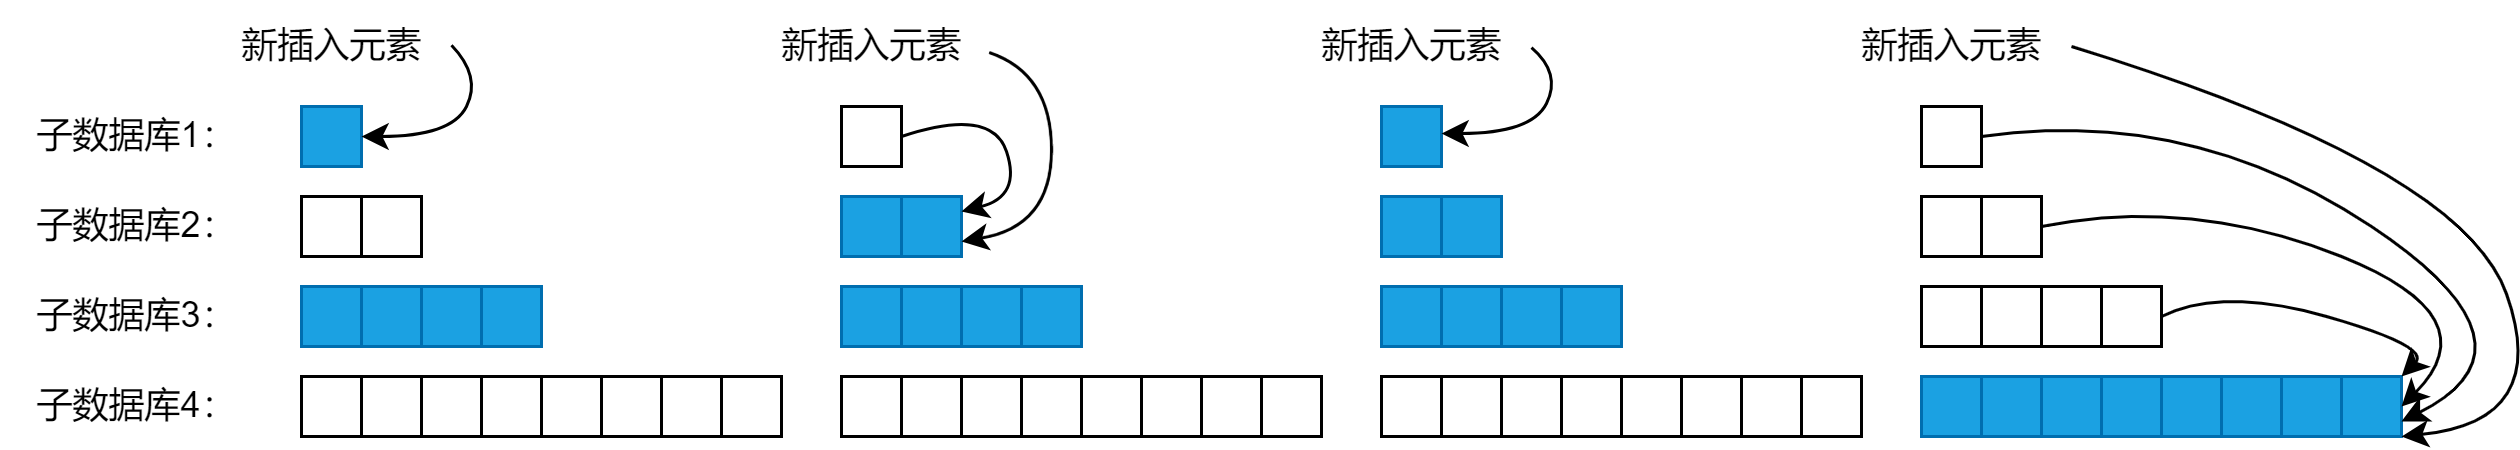
\includegraphics[width=0.8\linewidth]{figure/瀑布式插入.png}
    \caption{数据库插入示例}
    \label{fig:cascade-insertion}
\end{figure}

由于我们预先对数据库进行了分块,在插入时我们可以进行倍增操作。具体来说,如图\ref{fig:cascade-insertion}所示,每次插入都从最小的数据库(大小为$2^0$)开始,将其中一个空闲位置修改为插入的值。如果此数据库已满,就把这个数据库内的全部内容移动至下一个更大的数据库中,然后再重新尝试插入。对于每个内容有所变化的数据库,我们重新运行其对应的离线阶段。由倍增的性质,不难证明每次插入的均摊复杂度是对数级别的。

在实践中,我们可以考虑如下更简单的做法:将数据库分为两部分,静态数据与动态数据。于静态数据上运行本文提出的亚线性PIR协议,动态数据上运行任一不需要客户端存储数据库信息的线性PIR协议(如SealPIR\cite{SP:ACLS18}),每过一固定周期或当动态数据因新插入数据达到一定大小时,将静态数据与动态数据合并,重新运行亚线性PIR协议的预处理。